\documentclass{article}
\usepackage{graphicx}
\usepackage{hyperref}
\usepackage{enumitem}
\usepackage{datetime}
\usepackage{textcomp}

\usepackage{xcolor}


\begin{document}

\begin{tabular}{@{}ll}
    \textbf{\LARGE Hanxiao Liu} \newline
    \includegraphics*[draft,natwidth=85, natheight=34]{img/name-cn.png}
    \HCode{<script type="text/javascript" src="email.js"></script>} \newline
    1600 Amphitheatre Parkway \newline
    Mountain View, CA 94043
    &
    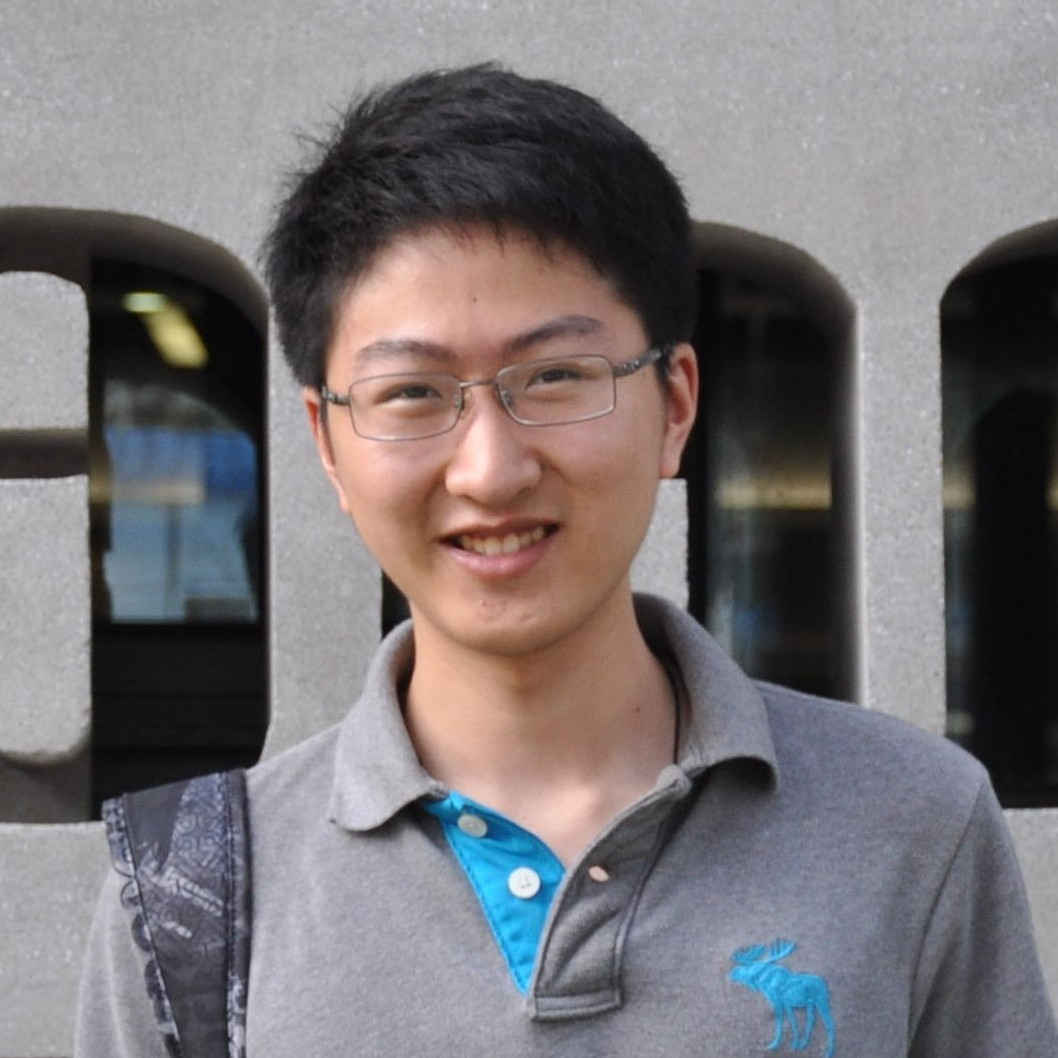
\includegraphics[natwidth=118, natheight=118]{img/profile.jpg} \\
\end{tabular}

\subsection*{README \ \ \ --- \protect
\href{https://github.com/quark0}{
\includegraphics[natwidth=22, natheight=22]{img/GitHub-Mark-64px.png}}
\href{https://scholar.google.com/citations?user=IMkVH_8AAAAJ&hl=en}{
\includegraphics[natwidth=22, natheight=22]{img/google-scholar.png}}
---
}
I'm a research scientist at \href{https://ai.google/research/teams/brain}{Google Brain}.
My interest is to build algorithms that learn to learn.

\noindent I received my Ph.D. from
the School of Computer Science at
\href{http://www.cmu.edu/index.shtml}{CMU},
working with Professor \href{http://www.cs.cmu.edu/~./yiming/}{Yiming Yang}.
Prior to that,
I received my B.E.\ from
Department of Automation at
\href{http://www.tsinghua.edu.cn/publish/newthuen/index.html}{Tsinghua University}.

\noindent Before joining Brain,
I interned at \href{https://deepmind.com/}{DeepMind} on neural architecture search.
I also spent time at \href{https://www.citadel.com/}{Citadel}, working on statistical arbitrage \& algorithmic trading.

\subsection*{}
\footnotesize{
    \textit{
        Last compiled on \today\ by \href{http://www.tug.org/tex4ht/}{\TeX4ht}. \newline
        Copyright \textcopyright\ \the\year\ Hanxiao Liu. All Rights Reserved.
    }
}

\end{document}
